\chapter{Debugging support}

\begin{quote}
  \textit{Debugging is twice as hard as writing the code in the first place.
    Therefore, if you write the code as cleverly as possible, you are, by
    definition, not smart enough to debug it.}\begin{flushright}
    \tiny{Brian W. Kernighan}
  \end{flushright}
\end{quote}

To debug programs written in a high level programming languages, we need the
compiler to emit debugging information. Without this information, we can still
debug programs at the assembly level. This can still be useful, for example for
reverse engineering. And, as was already hinted, source level debugging is
built upon assembly debugging. In this chapter, we describe at which level and
what kind of debugging support is provided. First, we will mention which kind
of mechanism the CPU itself offers. Going one step higher, we will talk about
the API that various operating systems provide. Finally, we'll discuss how are
compilers and debuggers able to allow us to debug source code although the
programs are still machine code programs. 

\section{CPU level support}
The CPU can only execute machine code which is made of instructions. It also
has several registers to help with computations. Which instructions and
registers the CPU has can differ from CPU to CPU. This is specified by
\textit{Instruction Set Architecture} (ISA) \cite{aps-isa}. It is an abstract
interface between the hardware and the lowest level software (machine code). It
contains all information needed to write a program in machine code. In general,
ISA specifies the following: 
\begin{itemize}
    \item Set of machine code instructions - Specifies instructions the ISA has
        and what operands each instruction has.
    \item Register set - Which registers the ISA has\footnote{Strictly speaking
        ISA doesn't have to use registers. It's possible to use only stack or
        accumulator, but most used ISAs use registers, so we'll ignore those
        architectures. }.   
    \item Addressing modes - Possible methods to refer to memory or register. 
\end{itemize}
This list is not exhaustive, for our purposes it is however enough. For each
instruction and operand it is specified how they should be encoded into binary.
CPU then \textit{implements} some ISA. If two different CPUs implement the same
ISA then they should be able to run the same machine code program. For example,
most PC use the \textit{x86} architecture \cite{aps-isa}, although the ARM
architecture is also seeing use in personal computers, for example, the Apple
Sillicon is of ARM architecture.

The x86 architecture is so called \textit{Complex Instruction Set Architecture}
(CISC). It contains many instructions that do many things at once, have varying
lengths, and take multiple clock cycles to complete \cite{intel-manual}. On the
other hand, the ARM architecture is \textit{Reduced Instruction Set
Architecture} (RISC). The number of instructions is smaller, they are intended
to be small building blocks from which complex operations may be created by
using many of them. Each instruction in RISC also has the same length. Both
architectures have their pros and cons, although some literature suggests that
in modern days the choice of architecture is irrelevant if one is only
considering performance and power consumption \cite{riscvscisc1, riscvscisc2}.
Unless specified otherwise the rest of this chapter will be talking about x86.
This is because T86 \todo{ref} is loosely based on x86, so it is most relevant
for us.

In the first chapter, we briefly mentioned that machine code programs can
instead be written in Assembly language. Assembly is almost 1:1 mapping to
machine code. When showing programs, we will show them in assembly. In figure
\ref{fig:assembly-example2}, we present another example of a program that was
compiled from C to assembly of the x86 architecture. As seen, instructions have
various operands. Most often registers (\texttt{RBP, RSP, EAX}), memory
(\texttt{[rbp-4]} is reference to memory at address which is in register
\texttt{rbp} minus $4$), or labels (like \texttt{L2}). Labels are not part of
machine code, instead memory address has to be provided. This is a small part
where assembly and machine code differ. For a detailed overview of the x86
instruction set see \cite{intel-manual}.

\begin{figure}\label{fig:assembly-example2}
    \begin{lstlisting}
max:
    push    rbp
    mov     rbp, rsp
    mov     QWORD PTR [rbp-24], rdi
    mov     DWORD PTR [rbp-28], esi
    mov     rax, QWORD PTR [rbp-24]
    mov     eax, DWORD PTR [rax]
    mov     DWORD PTR [rbp-4], eax
    mov     DWORD PTR [rbp-8], 1
    jmp     .L2
.L3:
    mov     eax, DWORD PTR [rbp-8]
    cdqe
    lea     rdx, [0+rax*4]
    mov     rax, QWORD PTR [rbp-24]
    add     rax, rdx
    mov     eax, DWORD PTR [rax]
    cmp     DWORD PTR [rbp-4], eax
    cmovge  eax, DWORD PTR [rbp-4]
    mov     DWORD PTR [rbp-4], eax
    add     DWORD PTR [rbp-8], 1
.L2:
    mov     eax, DWORD PTR [rbp-8]
    cmp     eax, DWORD PTR [rbp-28]
    jl      .L3
    mov     eax, DWORD PTR [rbp-4]
    pop     rbp
    ret
    \end{lstlisting}
    \caption{Compiled C program with GCC 9.4 compiler as x86 assembly.}
\end{figure}

\subsection{Registers}\label{subsection:registers}

The x86\_64 architecture has a set of general purpose registers.
Some of these are
\begin{itemize}
    \item RAX - Accumulator for operands and results data,
    \item RCX - Counter for string and loop operations,
    \item RSP - Stack pointer,
    \item RBP - Pointer to data on the stack.
\end{itemize}
Although there is a special role for each register, it is more of a convention.
It is not necessary to use RCX only for loop operations. Although the
\texttt{RSP} and \texttt{RBP} are called general purpose they are often only
used for pointing at the top of the stack, resp. to the base of the stack.
Stack is a special part of program memory with LIFO semantics. It can be used
to store the intermediate result, arguments to functions, return address, etc.
The \texttt{RBP} register is weird in a sense that it has this very special
purpose but is still considered part of the general purpose
registers~\cite{intel-manual}. One might use it for storing calculations, but
it would make the rest of the instructions that work with stack behave
unexpectedly.

The instruction pointer register (RIP on x86-64) contains the address of the
current instruction to be executed. As we mentioned in Introduction \todo{ref},
programs are executed sequentially from top to bottom, with certain
instructions having the ability to change the control flow. When an instruction
gets executed, the size of the instruction will be added to the value in RIP
register. This will advance the instruction pointer to the next instruction.
Or, if the instruction changes the control flow, the value in the instruction
pointer will be changed to the destination of the instruction. The register can
also be changed directly.

Another interesting register is the \texttt{EFLAGS} register. The register
contains a group of flags, which can alter various behavior of the CPU, or the
CPU itself sets them as a result of some instruction. For example the
instruction \texttt{cmp} compares its two operands and if they are the same the
\textit{zero} flag in the \texttt{EFLAGS} register will be set.

\subsection{Interrupts}
An interrupt is a special request to the CPU to stop the execution of the
current program and to quickly react to the reason that caused the request
\cite{aps-interrupts}. An example of such event can be a keyboard press or
error in a program (division by zero). There are two main categories
\cite{intel-manual}
\begin{itemize}
    \item An \textbf{interrupt} is an asynchronous\footnote{Meaning that the
        interrupt may happen when another instruction is being processed (not
        on the CPU clock edge).} event that is typically triggered by an
        Input/Output (IO) device.
    \item An \textbf{exception} is a synchronous event that is
        generated when the processor detects one or more predefined conditions
        when executing an instruction. These are further divided into three
        classes: faults, traps, and aborts.
\end{itemize}

For the rest of this thesis, we will use the word interrupt interchargebly for
both interrupt and exception although we will be mainly talking about
exceptions. This is to disambigous the exceptions which are at a programming
language level (like C++) and Microsoft structured exceptions about which we
will talk later. When an interrupt or exception happens, the processor halts
the execution of a current program and switches to a specific interrupt
handler. An interrupt handler is just another sequence of instructions that
gets executed when the interrupt happens. It is supposed to handle the
interrupt. An example of an exception is the \texttt{INT3} instruction. When
this instruction is executed an interrupt is generated. This instruction is
specifically meant to be used as a breakpoint. We can supply code that will be
responsible for handling the breakpoint as the interrupt handler. However, on
modern PCs, an Operating System (OS) is governing the PC. Alas, we cannot touch
the interrupt handler directly. Instead, an OS is going to have to provide
another layer of support for debugging.

Recall the EFLAGS register mentioned in section \ref{subsection:registers}.
There is a special flag called the trap flag. When it is set, the CPU will
issue an interrupt after every executed instruction. This could be useful if we
wanted to inspect execution instruction by instruction.

% Page ~3644 in intel manual
The CPU may also contain special debug registers. The x86 has six of them,
named DR0 to DR7, with DR4 and DR5 being synonyms for DR6 and DR7 on most CPUs,
otherwise they are reserved anyway. CPU provides special breakpoints through
these registers. The first four registers contain address of the breakpoints.
The debug status register \texttt{DR6} contains debug conditions that were
sampled at the last debug interrupt. Lastly, the debug control register
\texttt{DR7} is used to enable and disable breakpoints and set breakpoint
conditions. The CPU then issues an interrupt when these breakpoints are hit.
They can be triggered on memory read and write, on only on instruction
execution \cite{intel-manual}.

\subsection{Superscalar CPUs}
Modern CPUs do not execute instructions strictly one by one. They instead use
\textit{pipelines} and \textit{out-of-order execution}. This means that they
can execute several instructions at once and can execute them in non sequential
order. The observable behaviour of the program has to be the same as if it was
run sequentially. The CPU has to be careful about which instruction it can run
in parallel and out of order. The execution of an instruction consist of
several stages, which together form an \textit{execution pipeline}. The stages
can be \textit{Fetch}, \textit{Decode}, \textit{Execute}, \textit{Memory}, and
\textit{Writeback}, this may vary depending on architecture, but the general
ideas behind it are the same. The instruction must pass all these stages to be
successfully executed. To maximize efficiency, all stages are occupied by an
instruction. This means that when instruction $x$ leaves fetch stage, it goes
to the decode stage and instruction $y$ is put into the fetch stage.

However, when the next instruction is a conditional jump, there may be no way
to be sure if the jump will be taken.  CPUs deal with it in various ways and
try to predict the right branch. Sometimes however, the prediction fails and
the whole pipeline needs to be flushed. Same thing must happen when interrupt
occurs. The execution changes to the interrupt handler, the pipeline must
therefore be flushed because it contains instructions from the previous
location before the control flow was switched to the handler. Also, if we hit
the breakpoint, we want to make sure that instructions before it were all
executed and that none was executed after, otherwise it would be very confusing
for the user that tries to debug the program.

\section{Operating system support}
Operating system is a layer between computer components (CPU, memory,
input/output devices, \dots) and software. It is responsible for handling all
the resources so programmers do not have to think about it \cite{modern-os,
os-concepts}. Managing resources is not only to make writing programs easier
but to make sure that the programs are safe from each other. Modern operating
system allows to run multiple programs at once (or at least offer the illusion
that it can) and they make sure that one program cannot overwrite data or
otherwise interfere with other programs. Normal programs run in so-called
\textit{user space}, which has limited capabilities. The kernel on the other
hand runs in \textit{kernel space}. It has full access to the hardware of the
computer, can use all instructions, can permit or mask interrupts, and so on.

However, if programs were limited to user space all the time they would be very
limited. Sometimes, they need to escape the confinement of the OS, for example,
to read a file or communicate with other processes. Operating systems provide
an interface through which the user space program can leverage a small part of
the kernel in form of system calls. They offer a way of requiring some service
from the OS. This API is often in form of C and C++
functions~\cite{os-concepts}. A part of these functions is a special
instruction, like \texttt{SYSCALL} on x86~\cite{intel-manual}, that switches
the mode to kernel space. The kernel has to check if the call is correct since
it will be executed in kernel space with full access.

The most used operating systems today are Microsoft Windows, Linux, and MacOS.
Linux and MacOS systems are somewhat similar, but Windows is very different.

\subsection{Linux}\label{section:linux-dbg}
Linux offers a special system call which is very handy for debugging. It is
called \texttt{ptrace} \cite{ptrace} - process trace. It has following
signature: \texttt{ptrace(request, pid, void* addr, void* data)}. The request
is a \texttt{PTRACE\_COMMAND}, which specifies the behavior of the function
(for example \texttt{PTRACE\_SINGLESTEP}), pid of some process (presumably the
debugee) and two other parameters, whose meaning change depending on the
\texttt{PTRACE\_COMMAND} that was chosen\footnote{Peak API design!}. It allows
to observe and control the execution of another process, this process will be
the debugee. In the context of \texttt{ptrace}, we will instead use the word
tracee for the debugee, and tracer for the debugger, to be consistent with
ptrace documentation.

\texttt{ptrace} has many commands, here are some of the most important:
\begin{itemize}
    \item \texttt{PTRACE\_PEEKTEXT, PTRACE\_PEEKDATA} - Read tracee's memory,
    \item \texttt{PTRACE\_POKETEXT, PTRACE\_POKEDATA} - Write into tracee's
          memory,
    \item \texttt{PTRACE\_GETREGS} - Read tracee's register values,
    \item \texttt{PTRACE\_SETREGSET} - Modify tracee's register values,
    \item \texttt{PTRACE\_GETSIGINFO} - Retrieve information about the signal
                                        that caused tracee to stop,
    \item \texttt{PTRACE\_CONT} - Restart the stopped tracee process,
    \item \texttt{PTRACE\_SINGLESTEP} - Restart the stopped tracee but
          stop it after executing one instruction.
\end{itemize}

Linux however needs some way of notifying the debugger that the tracee
encountered a breakpoint, or that some other event requiring debugger attention
happened. To this end, \textit{signals} are used. They are in principle similar
to CPU interrupts. CPU interrupts are sent by the CPU and processed by the
operating system kernel. Signals are sent by the operating system kernel and
received by processes. They can also be sent by a process, that however happens
via system calls and so it goes through the kernel, so the statement still
stands. A signal is used in UNIX and Linux systems to notify a process that a
particular event has occurred \cite{os-concepts}.  When a process receives a
signal, it stops its execution and starts the execution of a signal handler.
There are various signal types. Most signals can have a custom signal handler
defined by the process. If no handler is defined then a default one is provided
by the OS. However, handlers for \texttt{SIGKILL} and \texttt{SIGSTOP} cannot
be changed \cite{signals}.

The reason for sending a signal to a process can be \todo{Tady toho asi bude vic}
\begin{itemize}
    \item CPU Interrupt (Division by zero, Breakpoint hit),
    \item System call (\texttt{kill(pid, signal)}).
\end{itemize}

For instance, the signal \texttt{SIGTERM} can be sent to a process to "ask it"
to exit. The process can handle this request, for example to save some state
before exiting. It can also however be completely ignored. For this, a signal
\texttt{SIGKILL} can be used, which cannot be handled, ignored, or blocked.

To begin tracing a command \texttt{PTRACE\_ATTACH} may be used for an already
existing process, or a \texttt{fork} followed with a child calling
\texttt{PTRACE\_TRACEME} and typically \texttt{execve}. When the tracee is
being traced it will stop each time a signal is delivered to it, even if it
chooses to ignore said signal. The tracer will be notified that the tracee
received a signal at its next call to the \texttt{waitpid} function. When the
tracee is stopped the tracer can initiate various ptrace requests listed above
to inspect and change the state of the tracee \cite{ptrace}.

In the CPU chapter, we mentioned that there are debug instructions and that
they issue an interrupt. We do not directly handle the interrupt here. Even if
we wanted, user space programs can't do that. The Linux kernel handles this for
us and instead uses the signals as an abstraction. \todo{Include kernel code.}

\subsubsection{Debugger implementation}
Now, we have all the necessary building blocks to build a simple debugger on
the Linux operating system running on the x86 platform. Running a program under
the debugger is simple. In figure \ref{fig:debugger-init} you can see the
initialization of the debugger. It uses the fork-exec idiom. \texttt{fork}
system call creates an exact copy of the process as a child except the
following: process ID (PID) of the child is different. In the parent process,
PID of the child is returned. In the child, $0$ is returned. In the child, we
initiate the \texttt{PTRACE\_TRACEME} call, which indicates that this process
is to be traced by its parent. Then it calls \texttt{execve} system call, which
replaces this program with the one we want to debug. The execve causes a
\texttt{SIGTRAP} signal on completion because it is being traced
\cite{execve}.

The parent first issues a \texttt{waitpid} system call. This waits for the
child \texttt{execve} to finish. The debugger then has a chance to debug the
child immediately, because it is stopped. The \texttt{while} loop can then
request input from the user and act accordingly. The tracee can be continued by
\texttt{PTRACE\_CONT} command.

\begin{figure}\label{fig:debugger-init}
    \begin{minted}{c}
        pid_t pid = fork();
        if (pid == 0) {
            // Begin tracing
            ptrace(PTRACE_TRACEME, 0, NULL, NULL);
            // Replace the code with the intended tracee code
            execve(executable, argv, NULL);
        } else {
            int w;
            waitpid(pid, &w, 0);
            while(...) {
                // Main debugger loop
            }
        }
    \end{minted}
    \caption{Linux - Debugger initialization.}
\end{figure}

Reading and writing to memory is simple. The \texttt{PTRACE\_PEEKTEXT} and
\texttt{PTRACE\_POKETEXT} are used for this purpose. This call reads or writes
a word (32 or 64 bits, depending on the Linux variant) into tracees memory.
However, if we want to write an arbitrary amount of bytes, we have to work
around the word limitation. We need to write by blocks and for the last one we
have to pad the write with already existing data if the block size does not
divide the word size. Figure \ref{fig:write-read} is shown how to read and
write exactly one byte of memory at a given address.

\begin{figure}\label{fig:write-read}
    \begin{minted}{c}
uint8_t read_memory(pid_t pid, uint64_t address) {
    uint64_t data = ptrace(PTRACE_PEEKDATA, pid, address, NULL);
    return (uint8_t)data;
}

void write_memory(pid_t pid, uint64_t address, uint8_t data) {
    uint64_t old_data = ptrace(PTRACE_PEEKDATA, pid, address, NULL);
    uint64_t new_data = (old_data & ~0xFF) | data;
    ptrace(PTRACE_POKEDATA, pid, address, new_data);
}
    \end{minted}
    \caption{Linux - Reading and writing one byte using ptrace.}
\end{figure}

Registers are similar to a memory in regards to how to read them. Linux
contains a predefined structure \texttt{user\_regs\_struct}, which maps all
registers on the current architecture. The command \texttt{PTRACE\_GETREGS}
then fills up this structure with the value in registers. To save registers,
\texttt{PTRACE\_SETREGS} can be used. One has to pass the whole structure, so
if we want to modify only some registers we first need to fetch the structure,
fill the registers we want with values, and then finally use \texttt{SETREGS}.
An implementation can be seen in figure \ref{fig:set-register}, the
\texttt{get\_register} functions maps the structure members to register name.
Since the address of the current instruction to be executed is also stored in a
register, we now have access to it.

\begin{figure}\label{fig:set-register}
    \begin{minted}{c}
void set_register(pid_t pid, const char* name, uint64_t data) {
    struct user_regs_struct regs;
    ptrace(PTRACE_GETREGS, pid, NULL, &regs);
    uint64_t* reg_data = get_register(&regs, name);
    *reg_data = data;
    ptrace(PTRACE_SETREGS, pid, NULL, &regs);
}
    \end{minted}
    \caption{Linux - Setting one register using ptrace}
\end{figure}

Breakpoints are more interesting. Debuggers often allow to enable and disable a
breakpoint, so we will distinguish between setting a breakpoint and enabling
it. Setting a breakpoint just means that the debugger needs to keep track of
where the breakpoint was set and if it is enabled or disabled. Enabling a
breakpoint means writing into the program memory the debug instruction (we will
use the x86 \texttt{INT3} with opcode \texttt{0xCC}). Figure
\ref{fig:with-and-without-bp} shows how code looks with and without enabled
breakpoint. On line $2$, the opcode changes from \texttt{0x83} to
\texttt{0xCC}. Since the breakpoint is set via the \texttt{PTRACE\_POKEDATA},
which only works data blocks, one has to pad the breakpoint opcode with already
existing data. Also, the rewritten data has to be kept so that the breakpoint
may later be deactivated. Abbreviated implementation can be found on
\ref{fig:breakpoint-enable}.

\begin{figure}\label{fig:with-and-without-bp}
    \begin{minipage}{0.45\textwidth}
        \begin{lstlisting}
c7 45 fc 05 00 00 00 	MOVL
83 7d fc 00          	CMPL
7e 07                	JLE
        \end{lstlisting}
    \end{minipage}
    \begin{minipage}{0.45\textwidth}
        \begin{lstlisting}
c7 45 fc 05 00 00 00 	MOVL
cc 7d fc 00          	INT3
7e 07                	JLE
        \end{lstlisting}
    \end{minipage}
    \caption{Code with and without breakpoint.}
\end{figure}

\begin{figure}\label{fig:breakpoint-enable}
    \begin{minted}{c}
void enable(pid_t pid, struct breakpoint* bp) {
    if (bp->enabled) {
        return;
    }
    bp->backup = read_memory(pid, bp->address);
    write_memory(pid, bp->address, BP_OPCODE);
    bp->enabled = true;
}

void disable(pid_t pid, struct breakpoint* bp) {
    if (!bp->enabled) {
        return;
    }
    write_memory(pid, bp->address, bp->backup);
    bp->enabled = false;
}
    \end{minted}
    \caption{Enabling breakpoints, abbr.}
\end{figure}

When a breakpoint is hit, the control is passed to the debugger, at this point,
the instruction pointer would point to the next instruction, which has opcode
\texttt{0x7D}, not \texttt{7E} (the \texttt{JLE} instruction) as might be
expected. This is because \texttt{INT3} is an instruction with size $1$. It
gets executed, the instruction pointer is advanced by the size ($1$) and an
interrupt is issued. But after the INT3 there were operands to the CMPL
instruction, we definitely do not want to interpret them as instruction. On
some architectures, advancing PC does not happen for the debug instruction
(like ARM \todo{Checked by hand - Reverse engineered from LLDB source code}.).

Additionally, if we just moved back and resumed the program, we would again hit
the breakpoint which is still set! We need to temporarily unset it, move one
instruction forward, and set it again. The general idea behind it can be found
in figure \ref{fig:continue}. With breakpoints, we essentially gained the
ability to single step as well. 

\begin{figure}\label{fig:continue}
    \centering
    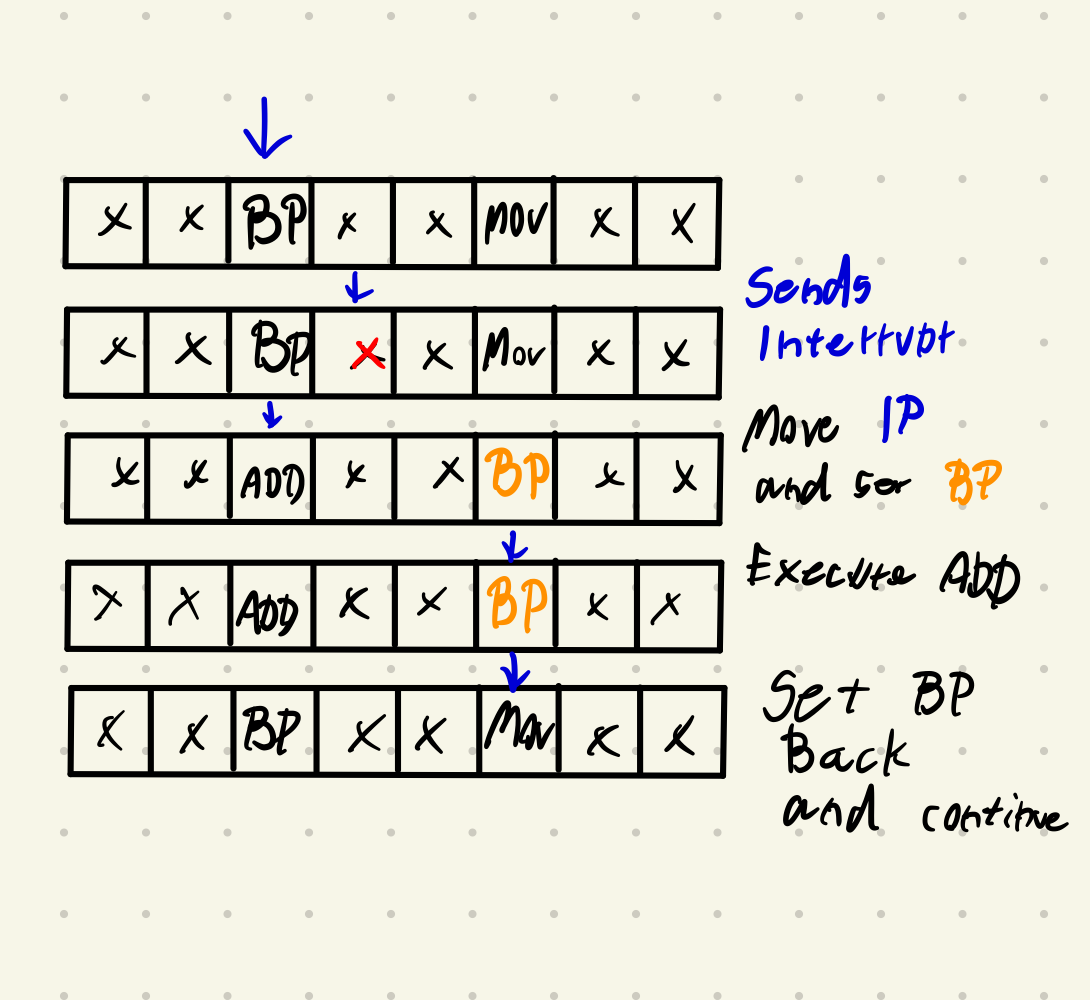
\includegraphics[width=100mm,scale=0.5]{media/breakpoint_tbd}
    \caption{Continue sketch}
\end{figure}

We showed that the breakpoint must be put at the next instruction. This is not
as simple as it sounds. Where is the next instruction? On CISC architectures,
this is not easy to find out since instructions have different sizes. But even
on RISC architectures like ARM, what if the instruction is a jump of some sort
and the next instruction is not simply the one that follows this one in the
code? For this reason, debuggers may need to have an instruction emulator,
which needs to emulate the whole instruction set to see where the program
counter ends up\footnote{And there can be a \textit{lot} of instructions
\cite{intel-manual}}. However, some architectures offer hardware support, like
the trap flag we mentioned in section \todo{ref}.

The ptrace library contains a special \texttt{PTRACE\_SINGLESTEP} command. This
executes one instruction in the tracee and then signal \texttt{SIGTRAP} will be
sent to it. The Linux kernel (as ofv6.1.8) uses the previously mentioned trap
flag for x86 \cite{linuxkernel-trapflag}. If the architecture does not provide
a way to support single stepping then the call will return an error. If we are
on an architecture that supports this command we can use it instead of the
register dance mentioned above. Implementation is described in figure
\ref{fig:singlestep}. We presume that the instruction pointer was moved when
the breakpoint was hit, so we do not need to return one byte backward. This is
more reasonable anyway since you want to show the user at which address was the
breakpoint hit. The LLDB \cite{lldb} debugger uses hardware support if there is
one, else it uses an instruction emulator. For example for the ARM
architecture, LLDB uses an instruction emulator. All instructions are of the
same length, however, some jump or another program counter modifier could cause
the next instruction to be executed is not necessarily the following one in the
code.

\begin{figure}\label{fig:singlestep}
    \begin{minted}{c}
void step_over_bp(pid_t pid) {
    uint64_t loc = read_register(pid, "rip");
    struct breakpoint* bp = find_bp(loc);
    if (bp == NULL || !bp->enabled) {
        return;
    }

    disable(pid, bp);
    ptrace(PTRACE_SINGLESTEP, pid, NULL, NULL);
    // Waits until debugee finishes singlestepping
    wait_for_debugee(pid);
    enable(pid, bp);
}
    \end{minted}
    \caption{Stepping over breakpoint, abbreviated.}
\end{figure}

For a normal single step, we can just use the \texttt{PTRACE\_SINGLESTEP}
command. We however need to check if the current line doesn't have a
breakpoint, since that would cause the debugger to return the program counter
back before it and we wouldn't be able to step over it. So, if there is a
breakpoint use the code from \texttt{fig:singlestep}, else just use
\texttt{PTRACE\_SINGLESTEP}.

Step over is more entertaining. It is used to jump out of the current function.
When a procedure is entered using the \texttt{call} instruction, the address
immediately after the call instruction is put onto the stack. Then, on entry to
the function, \texttt{rbp} register is pushed onto the stack and then the value
of it is set to the current value of the stack pointer. So the return address
is located at \texttt{rbp + 8}. We can set a breakpoint at that address and
then continue execution, wait for the debugee to hit the breakpoint, and then
disable and remove it. This has its flaws, for example, it won't work if the
step out is used before the rbp is set. Or if some library completely bypasses
the call instruction.

This concludes the implementation of a very basic assembly level debugger for
Linux on the x86 platform. The proof of concept implementation is provided as
an extension to this thesis and can be found under \todo{\texttt{<path to the
debugger>}}. The implementation was partially inspired by
\cite{linux-debugger-blog} and \cite{lldb}.

\subsubsection*{Hardware versus Software breakpoints}
The breakpoints we have implemented here are called \textit{software
breakpoints}. In section \todo{ref} we mentioned that CPU also supports
breakpoints, these are called \textit{hardware breakpoints}. The difference
between these two are mostly felt when doing reverse engineering, where people
study compiled programs in machine code because they do not have an access to
source code of the programs. This is done to find out what the program does,
for example to find out if it is of malicious nature. The programs themselves
however often try to defend from being debugged. Software breakpoints changes
the actual code, so a checksum of instruction opcodes can detect them. Hardware
breakpoints on the other hand do not touch the code, so they cannot be detected
as easily. They can also be used to break on memory access, which is not
possible with software breakpoints. However, we can only have limited number of
hardware breakpoints (4 on x86).

\todo{Describe how LLDB does things?}

\subsection{UNIX systems}
There are other systems based on UNIX, however, the implementation is very
similar to the Linux one. For example, MacOS, FreeBSD, and OpenBSD also have
the \texttt{ptrace} system call. The function is a little different on each
operating system but it can be used to achieve the same functionality as on the
Linux operating system.

\subsection{Windows}
The Microsoft Windows operating system also offers built-in support for
debugging. It is provided at the Win32 API layer
\cite{windows-msdn-debugging-api, windows-press-debugging-api}. It builds on
\textit{debug events} and \textit{debug functions}. Before we get to that
however, there is a need to signal and handle abnormal conditions which needs
to be immediately addressed, such as hitting a breakpoint or just interrupts in
general. The Linux and other POSIX compliant operating systems use signals,
which we have described in section \ref{section:linux-dbg}. Windows, however,
is not a POSIX system, and as such it uses a different strategy.

\subsubsection*{Structured Exception Handling}
Instead of signals, Windows uses \textit{Structured Exceptions}
\cite{windows-msdn-seh}. From now on, we will be using the abbreviation 'SEH'.
An exception is an event that requires the execution of code outside the normal
flow of control. There are software exceptions, like throwing an exception
explicitly or by the operating system, and hardware exceptions, which are
caused by the CPU (eg. interrupts). SEH unifies both of these things into one
just like signals do.

When an exception is triggered, control is transferred to the system. It saves
all necessary information that can later be used to continue execution from the
point where the exception was thrown. It also contains information about which
type of exception was thrown, if the execution can continue after handling the
exception, the address where the exception occurred and some other bits of
information\footnote{See MSDN documentation \cite{windows-msdn-seh} for full
detailed list}. The system then searches for an exception handler that will
handle the exception. The search is performed in this order:

\begin{enumerate}
    \item If the process is debugged the debugger is notified.
    \item If the process is not debugged or the debugger does not handle the
        exception, the frame-based exception handler is to be
        found\footnote{For detailed information about the handlers see
        \cite{windows-msdn-seh}.}
    \item If no frame-based handler can be found, or no handler handles the
        exception, but the process is being debugged then the debugger gets
        notified once again.
    \item The system provides a default handler, which often is the termination of
        the program via \mintinline{c}{ExitProcess}.
\end{enumerate}

The debugger has two opportunities to handle the exception. The
\textit{first-chance} is before the exception gets to the debugee. This is
intended for exceptions for which the debugger is responsible, for example,
breakpoint or single stepping. The debugger should handle these because the
debuggee is not responsible for them. The second opportunity, called
\textit{last-chance}, is when a debugee doesn't have an appropriate frame-based
handler to handle the exception. If the debugger weren't in the way, the system
would have already used the default exception handler, which is often program
termination. An example of an exception the debugger shouldn't handle on
first-chance is \texttt{EXCEPTION\_INT\_DIVIDE\_BY\_ZERO}. It should pass it
along to the debuggee. If however the debuggee does not have any appropriate
handler the debugger will get a last chance to look at the state of the program
before it will be killed \cite{windows-msdn-dbg-exc-handling}.

Two important exception types for debugging, both of which should be handled on
first-chance:
\begin{itemize}
    \item \texttt{EXCEPTION\_BREAKPOINT} - Raised when a breakpoint was encountered.
    \item \texttt{EXCEPTION\_SINGLE\_STEP} - Raised when a hardware-supported
        single step was completed.
\end{itemize}

\subsubsection{Debug events and functions}
Now that we have explained how a breakpoint may be signaled, let us look at
other tools that the Windows API gives us to allow for debugger implementation.
On Linux, we had a single function called \texttt{ptrace} which behavior
changed based on arguments. Windows on the other hand provides us with many
functions, some of which are:

\begin{itemize}
    \item \mintinline{c}{DebugActiveProcess} - Attaches the debugger to an
        active process.
    \item \mintinline{c}{DebugBreakProcess} - Causes a breakpoint exception to
        occur in the specified process. This passes control of the process to
        the debugger if there is one.
    \item \mintinline{c}{WaitForDebugEvent} - Waits for new debug events (on
        Linux, we used \texttt{waitpid}, which is more general purpose).
    \item \mintinline{c}{ContinueDebugEvent} - Continue the process execution
        after processing debug event (on Linux, we used the \texttt{PTRACE\_CONT}).
    \item \mintinline{c}{OutputDebugString} - Sends a string from the debuggee
        to the debugger.
    \item \mintinline{c}{ReadProcessMemory} and
    \mintinline{c}{WriteProcessMemory} - Read and modify process virtual
        address space. On linux we used \texttt{PTRACE\_PEEKTEXT} and
        \texttt{PTRACE\_POKETEXT}.
    \item \mintinline{c}{FlushInstructionCache} - Flushes instruction cache of
        the process. This should be used when modifying process text section,
        because the old instructions may still be cached.
\end{itemize}

The figure \ref{fig:win32debugger} depicts how a communication between
debugger, Windows and debugee can look. The debugger waits for debug events via
function \mintinline{c}{WaitForDebugEvent}. This function has a timeout
parameter, so the debugger can also do other things while it's waiting.

\begin{figure}
    \centering
    \scalebox{0.8}{
    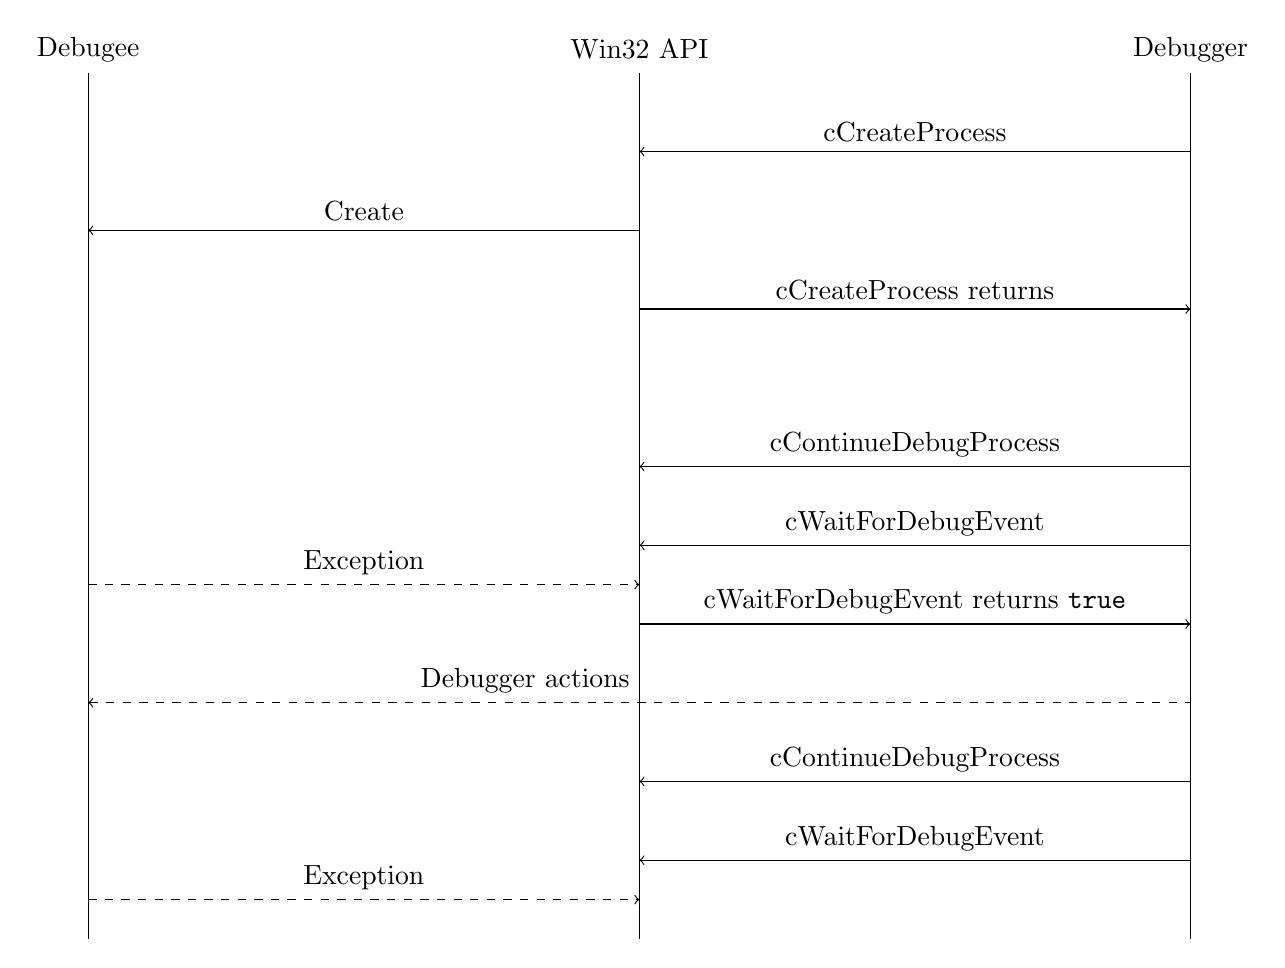
\begin{tikzpicture}
        \draw (-7,0) -- (-7,-11) (0,0) -- (0,-11) (7,0) -- (7,-11);
        \node at (-7,.3) {Debugee};
        \node at (0,.3) {Win32 API};
        \node at (7,.3) {Debugger};
        \draw[<-] (0,-1) -- node[midway,above] {\mintinline{c}{CreateProcess}} (7,-1);
        \draw[<-] (-7,-2) -- node[midway,above] {Create} (0,-2);
        \draw[->] (0,-3) -- node[midway,above] {\mintinline{c}{CreateProcess} returns} (7,-3);
        \draw[<-] (0,-5) -- node[midway,above] {\mintinline{c}{ContinueDebugProcess}} (7,-5);
        \draw[<-] (0,-6) -- node[midway,above] {\mintinline{c}{WaitForDebugEvent}} (7,-6);
        \draw[dashed,->] (-7,-6.5) -- node[midway,above] {Exception} (0,-6.5);
        \draw[->] (0,-7) -- node[midway,above] {\mintinline{c}{WaitForDebugEvent} returns \texttt{true}} (7,-7);
        \draw[dashed, <-] (-7, -8) -- node[above left] {Debugger actions} (7, -8);
        \draw[<-] (0,-9) -- node[midway,above] {\mintinline{c}{ContinueDebugProcess}} (7,-9);
        \draw[<-] (0,-10) -- node[midway,above] {\mintinline{c}{WaitForDebugEvent}} (7,-10);
        \draw[dashed,->] (-7,-10.5) -- node[midway,above] {Exception} (0,-10.5);
    \end{tikzpicture}
    }
    \caption{A sequence diagram for debugger using Windows API. Inspired by
             \todo{NI-REV 6. lecture}}
    \label{fig:win32debugger}
\end{figure}
 
\subsubsection*{Debug Events}\label{section:Debug Events}
Debugging events are various incidents in the debuggee that causes the system
to notify the debugger \cite{windows-msdn-debug-events}. These are stored in
special \mintinline{c}{DEBUG_EVENT} structure, which is received in
\texttt{WaitForDebugEvent} call initiated from the debugger. This structure
contains various information about the event, the internals can be seen in
figure \ref{fig:DebugEvent}. These events include loading and unloading a DLL,
creating and exiting a process, sending debug strings via the
\mintinline{c}{OutputDebugString}, and last but not least, exception occurence.
Exceptions include the \texttt{EXCEPTION\_BREAKPOINT} and
\texttt{EXCEPTION\_SINGLESTEP} mentioned previously, which are vital to the
debugger.

\begin{figure}
\begin{minted}{c}
typedef struct _DEBUG_EVENT {
  DWORD dwDebugEventCode;
  DWORD dwProcessId;
  DWORD dwThreadId;
  union {
    EXCEPTION_DEBUG_INFO      Exception;
    CREATE_THREAD_DEBUG_INFO  CreateThread;
    CREATE_PROCESS_DEBUG_INFO CreateProcessInfo;
    EXIT_THREAD_DEBUG_INFO    ExitThread;
    EXIT_PROCESS_DEBUG_INFO   ExitProcess;
    LOAD_DLL_DEBUG_INFO       LoadDll;
    UNLOAD_DLL_DEBUG_INFO     UnloadDll;
    OUTPUT_DEBUG_STRING_INFO  DebugString;
    RIP_INFO                  RipInfo;
  } u;
} DEBUG_EVENT, *LPDEBUG_EVENT;
\end{minted}
\caption{Structure which contains info about debug event.}
\label{fig:DebugEvent}
\end{figure}

\subsubsection*{Tying it all together}
Now we have all necessary building blocks to create ourselves a tiny Windows
compiler. The implementation itself would be very similar to the Linux one we
presented in section \ref{section:linux-dbg}. To provide at least some idea,
figure \ref{fig:windows-debugger-mainloop} contains an abbreviated main loop of
the debugger \cite{windows-msdn-dbg-main-loop}. We not only need to handle
exception debug events but others also if we want our debugger to be robust.
For example, thread creation might interest us too, so that we can trace all
threads of the debugee.

\begin{figure}\label{fig:windows-debugger-mainloop}
    \begin{minted}{c}
void EnterDebugLoop(const LPDEBUG_EVENT DebugEv)
{
   DWORD dwContinueStatus = DBG_CONTINUE; // exception continuation
   for(;;)
   {
      WaitForDebugEvent(DebugEv, INFINITE);
      switch (DebugEv->dwDebugEventCode)
      {
            case EXCEPTION_ACCESS_VIOLATION: 
               // First chance: Pass this on to the system.
               // Last chance: Display an appropriate error.
                  break;

               case EXCEPTION_BREAKPOINT:
               // First chance: Display the current
               // instruction and register values.
                  break;

              // Other exception types like singlestep ...
              ...
          }
          // Other debug events
          ...
      }
   ContinueDebugEvent(DebugEv->dwProcessId,
                      DebugEv->dwThreadId,
                      dwContinueStatus);
   }
}
    \end{minted}
    \caption{An abbreviated example of a Windows Debugger loop, taken from \cite{windows-msdn-dbg-main-loop}}
    % Beware, this figure is cursed. Adding caption here will break the entire
    % build for god knows what stupid reason. If it works add citation
    % to Writing main debugger loop.
\end{figure}

\section{Source Level Debugging}
If we want to debug at the source code level, we need to give the debugger some
information, because otherwise, it can only work with the generated machine
code. For instance, we somehow need to provide information to the debugger that
the instruction at address \textit{0xABCD} belongs to line \texttt{5} in the
source code. Or we need to provide information about where is some variable
located. Before we get into that, we will take a brief look at the layout of
executables and where are those pieces of debugging information stored.

\subsection{Executable file formats}
ELF is one of the executable file formats. The abbreviation ELF means
Executable and Linkable format. The file itself consists of sections, some of
which are
\begin{itemize}
    \item .text - the executable code,
    \item .data - allocated space and values of initialized static\footnote{In
        this context, static means that the variable exists for the entire
        lifetime of the program.} variables and other objects,
    \item .bss - allocated space for uninitialized static variables,
    \item .rodata - data that doesn't change for the entirety of the program
        lifetime, like strings literals in C.
    \item various debug sections like .debug\_info, .debug\_line etc.
\end{itemize}
For inspecting the ELF files, commands \texttt{readelf} and \texttt{objdump}
may be used on Linux systems. The ELF format also has a header, and all
sections have their header too. This contains information like the name of the
section, the size of the section, etc. The ELF format are not only used for
executables, but also for \textit{relocatable} file, \textit{executable} file
and \textit{shared object} file \cite{elf}. The sections themselves are often
protected. For example, the .text section can only be read and executed, but
cannot be written into. The .data section can be read and written, but cannot
be executed. We also see that the ELF contains various debug sections, so the
debugging information is embedded in the executable itself.

ELF is not the only one executable format. Others include the \textit{COFF} and
\textit{PE} format, which is used by Microsoft Windows, or the \textit{Mach-O},
which are mostly used on the MacOS operating system. Interesting distinction is
that the Mach-O saves debugging information into separate file with extension
\texttt{dSYM}. One possible encoding of this debugging information is specified
by a DWARF standard.

\subsection{DWARF}
DWARF\footnote{The name DWARF is a pun since it was developed alongside ELF.}
is a debugging format used to describe programs written in procedural
languages. It is primarily associated with the ELF file format. It aims to
support all different types of information that may be needed while debugging.
It also strives to encode this information in as much space efficient manner as
possible. This can make it somewhat complex. 

There are five versions of the standard, we will be mainly talking about
version 2, since the others mainly add features to accommodate newer language
features. We will not get that far even in version 2. The complete changelog
can be found in the text describing DWARF version 5 \cite{dwarf-5}. We provide
many examples of the information that DWARF encodes. For reading the DWARF
information from object files, we used the \texttt{llvm-dwarfdump},
\texttt{objdump}, and \texttt{readelf} tools. The information DWARF encodes is
stored in various debug sections if used in conjunction with the ELF standard.
If with Mach-O, it is stored in separate file. This file is still however split
into several sections.

\subsubsection{Line Number Information}
Line number information needs to convey which line of code corresponds to an
address of machine code instruction. The DWARF standard \cite{dwarf} mentions
that encoding this information would be possible in a matrix, which would have
one row for each instruction. The columns of the matrix would contain
\begin{itemize}
    \item the source file name,
    \item the source line number,
    \item the source column number,
    \item whether this instruction is the beginning of a source statement,
    \item whether this instruction is the beginning of a basic
        block\footnote{Basic block is a sequence of instructions that is
        entered only at the first instruction and exited only at the last
        instruction \cite{dwarf}. In other words, all of the instructions in
        the basic block are executed sequentially.}
\end{itemize}
They however argue that such a matrix would be very big. The matrix is
therefore stripped of redundant information. For instance, instruction whose
location is the same as the previous one is removed. Instead of a matrix, they
provide a virtual machine specification and a bytecode language that one has to
interpret to reconstruct this matrix and consequently to get the necessary
debugging information.

The virtual machine consists of registers \texttt{address}, \texttt{file},
\texttt{line}, \texttt{column}, \texttt{is\_stmt}, \texttt{basic\_block}, and
\texttt{end\_sequence}. The program itself begins with a prologue. This
prologue contains the length of the program, version, length of the prologue,
length of instructions (so that it may be better compressed), and similar
pieces of information. 

Then the \textit{Standard opcodes} are provided, which are instructions of the
virtual machine. These are mostly used for manipulating the registers of the
machine or to create a row from the values in the registers and append it to
the matrix \cite{dwarf}. 

It also has several \textit{Special opcodes}, each of which does the following
operations:
\begin{itemize}
    \item Add a signed integer to the \texttt{line} register.
    \item Multiply an unsigned integer by the smallest length of instruction
        and add the result to the \textit{address} register.
    \item Append a row to the matrix consisting of the current values in
        registers.
    \item Set the \texttt{basic\_block} register to false.
\end{itemize}
All of these opcodes always do these four operations, they only differ in what
values they add to the \texttt{line} and \texttt{address} register
\cite{dwarf}. Those values are calculated from the instruction opcode, which
ranges from $10$ to $255$ in DWARF version 2. This is the most common series
of operations the virtual machine must do. Encoding it into single opcode 
makes the program extremely size efficient.

Observe the program in figure \ref{fig:c-program-and-its-assembly}. A simple
greeter-like program that displays the name given to it as an argument. With
the \texttt{readelf} utility program, we can inspect the DWARF bytecode
language describing the locations, it is showed in figure \ref{fig:dwarf-locations}. 
First few lines of the example are explained below, we ignore the set column which
is only used for the location to be precise.
\begin{itemize}
    \item \texttt{0x41} - Jump to the beginning of main function (ie. \texttt{0x1139}).
    \item \texttt{0x4c} - Special opcode - Increment line by one and advance
        address by zero. Although the advance address was essentially a noop it
        was still more space efficient to use special opcode, because the
        \texttt{advance\_pc} instruction DWARF offers would take up at least
        two bytes (the opcode and the operand), whereas
        the special opcode occupies only one.
    \item \texttt{0x4f} - Special opcode - Increment line by 2 to 3 and advance address by 15 to \texttt{0x1148}.
        This essentialy skips the function prologue and advances to instruction \texttt{cmpl}, which represents
        line \mintinline{c}{if(argc < 1)} of the program.
    \item \texttt{0x52} - Special opcode - advance line by 1 to 4 and advance address by 6 to \texttt{0x114e}.
        This is the \mintinline{c}{return 1;} line of the program.
\end{itemize}
Remember that each of the special opcode also creates a line in the matrix. As
said, this is extremely space efficient. DWARF stores this encoded information
in section \texttt{.debug\_line}.

\begin{figure}
    \begin{minted}{c}
#include <stdio.h>
int main(int argc, char* argv[]) {
    if (argc < 1)
        return 1;
    const char* name = argv[1];
    printf("Hello, %s\n!", name);
    return 0;
}
    \end{minted}
    \begin{lstlisting}
0000000000001139 <main>:
    1139:	55                   	push   %rbp
    113a:	48 89 e5             	mov    %rsp,%rbp
    113d:	48 83 ec 20          	sub    $0x20,%rsp
    1141:	89 7d ec             	mov    %edi,-0x14(%rbp)
    1144:	48 89 75 e0          	mov    %rsi,-0x20(%rbp)
    1148:	83 7d ec 00          	cmpl   $0x0,-0x14(%rbp)
    114c:	7f 07                	jg     1155 <main+0x1c>
    114e:	b8 01 00 00 00       	mov    $0x1,%eax
    1153:	eb 2c                	jmp    1181 <main+0x48>
    1155:	48 8b 45 e0          	mov    -0x20(%rbp),%rax
    1159:	48 8b 40 08          	mov    0x8(%rax),%rax
    115d:	48 89 45 f8          	mov    %rax,-0x8(%rbp)
    1161:	48 8b 45 f8          	mov    -0x8(%rbp),%rax
    1165:	48 89 c6             	mov    %rax,%rsi
    1168:	48 8d 05 95 0e 00 00 	lea    0xe95(%rip),%rax
    116f:	48 89 c7             	mov    %rax,%rdi
    1172:	b8 00 00 00 00       	mov    $0x0,%eax
    1177:	e8 b4 fe ff ff       	call   1030 <printf@plt>
    117c:	b8 00 00 00 00       	mov    \$0x0,%eax
    1181:	c9                   	leave
    1182:	c3                   	ret
    \end{lstlisting}
    \caption{A program in C and corresponding program in assembly.}
    \label{fig:c-program-and-its-assembly}
\end{figure}

\begin{figure}
    \begin{lstlisting}
[0x3f] Set column to 34
[0x41] Extended opcode 2: set Address to 0x1139
[0x4c] Special opcode 6: advance Address by 0 to 0x1139 and Line by 1 to 2
[0x4d] Set column to 8
[0x4f] Special opcode 216: advance Address by 15 to 0x1148 and Line by 1 to 3
[0x50] Set column to 16
[0x52] Special opcode 90: advance Address by 6 to 0x114e and Line by 1 to 4
[0x53] Set column to 17
[0x55] Special opcode 104: advance Address by 7 to 0x1155 and Line by 1 to 5
[0x56] Set column to 5
[0x58] Special opcode 174: advance Address by 12 to 0x1161 and Line by 1 to 6
[0x59] Set column to 12
[0x5b] Advance PC by constant 17 to 0x1172
[0x5c] Special opcode 146: advance Address by 10 to 0x117c and Line by 1 to 7
[0x5d] Set column to 1
[0x5f] Special opcode 76: advance Address by 5 to 0x1181 and Line by 1 to 8
[0x60] Advance PC by 2 to 0x1183
[0x62] Extended opcode 1: End of Sequence
    \end{lstlisting}
    \caption{A DWARF description of mapping source lines to addresses for
    program in figure \ref{fig:c-program-and-its-assembly}.}
    \label{fig:dwarf-locations}
\end{figure}

\subsubsection{Debugging Information Entry}
The \textit{Debugging Information Entries}, or DIEs, are the building blocks of
debugging information in DWARF. Each DIE has a tag and a series of attributes.
The tag specifies the class to which an entry belongs, like
\texttt{DW\_TAG\_subprogram}, which is used for functions, or
\texttt{DW\_TAG\_variable}, which is used for variables. A complete list can be
found in \cite{dwarf}. Those entries can be found in \texttt{.debug\_info}
section \cite{dwarf}. 

The attributes themselves then convey some property of the DIE, like the name
and type of a variable or starting and ending address of a function. The DIEs
form a tree-like structure. Each DIE is owned by one parent (excluding the top
DIE) and can own multiple DIEs. These relations somewhat mimic the relations of
the program structures. For instance, variable is owned by a function in which
it was defined. There are also other relations among the DIEs, not only
ownership. With those relations in place, the relation is a graph, not just a
tree.

An example of DWARF DIEs can be seen in figure \ref{fig:dwarf-die}. The
\texttt{DW\_TAG\_pointer\_type} is simple, its attributes are only the size of
the type and which type it points to, this is encoded as an address to another
DIE. The type it points to is another DIE. It only contains information that
its a const type, and again has a link to another DIE. Finally, the die at
\texttt{0x6b} has a base type. It contains the size of the type, name, and
encoding. 

We also have the \texttt{DW\_TAG\_SUBPROGRAM}, which represents a function. It
has many attributes, like name, path to the file where it was declared, on
which line and column it is located, at which machine code address the function
begins and ends, and so on. This DIE also owns some other DIEs (indicated by
indentation). Here, the children are the parameters and variables of the
function. Important information about variables is where they are stored, so
that we may look up their value. We can also see that the variable
\texttt{name} has an attribute type, which points to the DIE at address
\texttt{0x8f}, which is the DIE we were talking about previously.

\begin{figure}
    \begin{lstlisting}
0x6b: DW_TAG_base_type
        DW_AT_byte_size (0x01)
        DW_AT_encoding (DW_ATE_signed_char)
        DW_AT_name ("char")

0x72: DW_TAG_const_type
        DW_AT_type (0x0000006b "char")

0x8f: DW_TAG_pointer_type
        DW_AT_byte_size	(8)
        DW_AT_type (0x00000072 "const char")

DW_TAG_subprogram
  DW_AT_external	(true)
  DW_AT_name	    ("main")
  DW_AT_decl_file	("/home/gregofi1/tmp/main.c")
  DW_AT_decl_line	(2)
  DW_AT_decl_column	(0x05)
  DW_AT_prototyped	(true)
  DW_AT_type        (0x00000058 "int")
  DW_AT_low_pc      (0x0000000000001139)
  DW_AT_high_pc	    (0x0000000000001183)
  DW_AT_frame_base	(DW_OP_call_frame_cfa)
  DW_AT_call_all_tail_calls	(true)
  DW_AT_sibling	    (0x000000e0)

    DW_TAG_formal_parameter
      DW_AT_name	    ("argc")
      DW_AT_decl_file	("/home/gregofi1/tmp/main.c")
      DW_AT_decl_line	(2)
      DW_AT_decl_column	(0x0e)
      DW_AT_type	    (0x00000058 "int")
      DW_AT_location	(DW_OP_fbreg -36)

    DW_TAG_formal_parameter
      DW_AT_name	    ("argv")
      ...

    DW_TAG_variable
      DW_AT_name	    ("name")
      DW_AT_decl_file	("/home/gregofi1/tmp/main.c")
      DW_AT_decl_line	(5)
      DW_AT_decl_column	(0x11)
      DW_AT_type	    (0x0000008f "const char *")
      DW_AT_location	(DW_OP_fbreg -24)
    \end{lstlisting}
    \caption{A part of DWARFs DIEs for program in figure \ref{fig:c-program-and-its-assembly}}
    \label{fig:dwarf-die}
\end{figure}

\subsubsection{Locations of variables}
Locations are probably the most complicated thing in the DWARF standard. Like
with locations, a virtual machine is needed to decode this information.
Variables are generally stored in one place. This can be a memory, register, or
stack. Sometimes however the location of an object can change throughout its
lifetime, it may not be present at all since it was optimized away, it can be
split into several locations, or it might be a reference to some other object.
The fact that an object changes location throughout its lifetime seldom happens
\cite{dwarf-intro}, but DWARF is nevertheless prepared for it \cite{dwarf}.

Contrary to the virtual machine described in line encoding, which was
register-based, this one is stack-based. This means that most operations take
their operands from the stack and push the result back onto the stack. More
about stack-based virtual machines can be discovered in
\cite{crafting-interpreters}. DWARF calls those instructions
\textit{expressions} \cite{dwarf}. The last value on the top of the stack after
the VM runs is considered to be the resulting value (this can be an address of
an object, value of an array bound, length of dynamic string, and so on)
\cite{dwarf}. For example in the figure \ref{fig:c-program-and-its-assembly}
there is the \texttt{DW\_OP\_fbreg -24}, this pushes value at offset $-24$ by
the register specified by a descriptor in \texttt{DW\_AT\_frame\_base}, which
often is a base pointer to the stack. And since there are no more expressions
the computed value on the top of the stack is the resulting location of the
variable that the debugger will get to use.

There are many types of expressions, like arithmetic operations, stack
manipulation, control flow operations, and last but not least, the
specifications of the location. We provided already the example with the base
pointer to the stack, let us look at some more examples, mostly taken from
\cite{dwarf}:
\begin{itemize}
    \item \texttt{DW\_OP\_reg3} - The value is in register $3$.
    \item \texttt{DW\_OP\_addr 0xABCD} - The value of a static variable is at
        address \texttt{0xABCD}.
    \item \texttt{DW\_OP\_bregx 54 3; DW\_OP\_deref} - Adds $54$ to value in
        register $3$. This should yield an address. The value at the location
        to which address points is then pushed onto the stack. This can be used
        for recording information about references and pointers.
    \item \texttt{DW\_OP\_reg3; DW\_OP\_dup; DW\_OP\_add} - Fetches value from
        register $3$ and pushes it onto the stack, duplicates that value and
        pushes it on the stack, and pops two values from the stack, adds them
        together, and pushes them back onto the stack\footnote{Artificial
        example just to show the power of the language.}.
\end{itemize}
With this computational power, we can save any information we need. There are
many more instructions, all of which can be found in \cite{dwarf}. An example
of an interpreter for this can be found in the LLDB source code in file
\texttt{source/Expression/DWARFExpression.cpp}.

\subsubsection{Call frames}
Debuggers often need to know through which function calls the executed program
went to arrive at a certain state \cite{dwarf}. For each function call, there
is a \textit{stack frame} saved on the stack. Stack frame is a part of the stack memory that
contains information relevant to the function invocation. An example of a
stack frame can be seen in figure \ref{fig:stack-layout}.
Stack frames mostly consist of the following:
\begin{itemize}
    \item Return address - This contains the location from which the program
        was called so that after the function finishes it may properly return
        to that location. This fact was also used in our step-out
        implementation in \ref{section:linux-dbg}.
    \item Base pointer backup - Backup of the value in the base pointer which
        was set by the previous function. This register needs to be preserved
        between calls, that's why a backup is made. Other registers might need
        to be saved for the same reason.
    \item Allocated space for variables - A space for local variables.
\end{itemize}
Stack frames are described in more detail in \cite{dragon-book}, where they are
called activation records. We also provide an example of how a function
prologue and epilogue look, so one may get a better feel about how such stack
frame comes to fruition \ref{fig:prologue-and-epilogue}.

Debuggers need to do a so-called stack unwinding. Unwinding essentially means
going to a state where the previous stack frame is the most recent. This needs
to be done several times to get the whole chain of function calls which led to
the current state of the program. We could relatively simply get to the
previous stack frame. But to get to the previous one is not easy. We need to
know exactly where was the base pointer and possibly other registers saved so
that we may simulate the unwinds.

DWARF proposes a table, in each row, there is an address of a location in the
program, a location of a stack frame, and values of other registers for that
location. However, such table would be very large, so DWARF again uses a
virtual machine for the construction of the table, since many columns in one
row would be have the same values in the following rows \cite{dwarf}. The
location of a stack frame can be described either by a register and a signed
offset which are added together, or a DWARF expression may be used (the ones
used to describe variable locations).

Figure \ref{fig:dwarf-stack-frames} contains an example of the encoding of this
information and also the decoded values for the program in figure
\ref{fig:prologue-and-epilogue}. The \texttt{advance\_location} adds a new row
to the matrix, with the only thing changing from the previous row being the
location value. The \texttt{def\_cfa\_offset} specifies that the CFA (current
stack frame) is at the provided offset from the same register it was offseted
in previous row. We can see that in the example on line $2$ the offset changes
from $8$ to $16$, but the register stays the same. This is apparent in the
decoded information where on the address \texttt{0x1184} the \texttt{CFA}
changed from \texttt{RSP + 8} to \texttt{RSP + 16}. This happened because
the \texttt{push \%rbp} advanced the stack pointer by eight bytes.

On the contrary, the \texttt{def\_cfa\_register} changes the register but keeps
the offset. This happens when the instruction \texttt{mov \%rsp, \%rbp} is
executed. From that point the stack frame is at sixteen byte offset from the
base pointer. This holds until the epilogue, where the old stack pointer is
restored. In the example in the decoded information, many more registers were
missing. This is because their value didn't change across the function, so
there was no need to save information about them.

The DWARF offers more instructions for manipulation, for a complete overview
and another example consult \cite{dwarf}. With this information, DWARF can
describe a way to simulate a stack unwinding without touching the state of the
debugee.

\begin{figure}
    % In case supervisor will want the opcodes in binary then just use git
    % history!
    \begin{lstlisting}
0000000000001183 <foo>:
0x1183:	push   %rbp          ; Save old stack frame pointer
0x1184:	mov    %rsp,%rbp     
0x1187:	sub    \$0x18,%rsp   ; Allocate space on the stack
                                <body ...>
0x11b1:	leave                ; deallocate and restore regs
0x11b2:	ret
    \end{lstlisting}
    \caption{A prologue and epilogue of a function in assembly.}
    \label{fig:prologue-and-epilogue}
\end{figure}

\begin{figure}
    \begin{lstlisting}
... FDE cie=00000000 pc=00001183...000011b3
DW_CFA_advance_loc: 1
DW_CFA_def_cfa_offset: +16
DW_CFA_offset: RBP -16
DW_CFA_advance_loc: 3
DW_CFA_def_cfa_register: RBP
DW_CFA_advance_loc: 43
DW_CFA_def_cfa: RSP +8

0x1183: CFA=RSP+8: RIP=[CFA-8]
0x1184: CFA=RSP+16: RBP=[CFA-16], RIP=[CFA-8]
0x1187: CFA=RBP+16: RBP=[CFA-16], RIP=[CFA-8]
0x11b2: CFA=RSP+8: RBP=[CFA-16], RIP=[CFA-8]
    \end{lstlisting}
    \caption{A DWARF stack frame information about the program in
             \ref{fig:prologue-and-epilogue}. Top part contains the encoded
             program for virtual machine, bottom part contains the decoded
             table from interpreting the program. Abbreviated.}
    \label{fig:dwarf-stack-frames}
\end{figure}

% Inspired from
% https://tex.stackexchange.com/questions/583197/
% how-can-i-put-two-boxes-right-next-to-each-other-that-have-the-exact-same-size
\begin{figure}
    \begin{tikzpicture}[
node distance = 0pt,
square/.style = {draw=black!60, fill=white!5, very thick, 
                 minimum height=1.6cm,
                 outer sep=0pt,
                 trapezium stretches=true}, % To make all nodes of the same height
]
        \node (pro2) [square,
                      text width=3cm] {Return address (8B)};
        \node (pro3) [square,
                      right=of pro2,
                      text width=3cm] {BP backup (8B)}; 
        \node (pro4) [square, right=of pro3,
                      text width=3cm] {Potential backup of other registers}; 
        \node (pro5) [square, right=of pro4,
                       text width=3cm] {Allocated space for variables}; 
    \end{tikzpicture}
    \caption{Basic stack layout after function prologue, disproportional.}
    \label{fig:stack-layout}
\end{figure}

\subsubsection{Other informations}
The DWARF standard has information about compilation units, since object files
may be derived from multiple compilation units \cite{dwarf}. It also has
information about subroutines and inlined subroutines, lexical blocks,
try-and-catch blocks, and many other constructs. These are not special in any
way, we have seen a small example in figure \ref{fig:dwarf-die}. They mainly
store the beginning and end and some other information. They also contain
various information about macros, so that the debugger can work with the
original code before the macro expansion.

It also contains many type entries.
Those are split into different categories, we present some of the most common:
\begin{itemize}
    \item Base types - Provided by the language, like \texttt{int},
        \texttt{char}.
    \item Modifier types - Modifies some existing type, like type qualifiers
        from C (\texttt{const}, \texttt{volatile} and \texttt{mutable}), or
        pointers.
    \item Array types - A sequential storage space containing objects of the
        same type. Multidimensional arrays are considered a special type.
        An interesting attribute that a multidimensional array has is ordering -
        either column-wise or row-wise. This is not relevant to C, since it has no
        notion of a multidimensional array.
    \item Structure, Union, and Class types - User-defined types that pack
        together several different types. Information is provided about the
        members, especially the bit offset at which they reside in the structure
        and in which order were they declared. In addition, the size of the type
        is specified - if it can be determined at compile time (In C, it cannot
        be determined for forward declarations). For C++, information about
        inheritance, like deriving, accessibility, and if the inheritance is
        virtual, is provided.
    \item Enumeration type.
    \item Subroutine type - Used for types of functions in C. However, for the
        functions themselves, their type is specified as return type. Types of
        their parameters are specified in the parameters themselves since they
        are DIEs and are children of the function. We showed this in the figure
        \ref{fig:dwarf-die}. This subroutine type is for example used if one
        would create a pointer to a function. Then the type of that is a pointer
        to the subroutine type. An abbreviated example can be seen on
        \ref{fig:dwarf-ptr-to-fun}.
\end{itemize}

\begin{figure}
    \begin{lstlisting}
0x138:   DW_TAG_subroutine_type
            DW_AT_type	(0x00000131 "int")
            DW_AT_sibling	(0x14c)

0x141:     DW_TAG_formal_parameter
              DW_AT_type	(0x131 "int")

0x146:     DW_TAG_formal_parameter
              DW_AT_type	(0x14c "double")

0x153:   DW_TAG_pointer_type
            DW_AT_byte_size	(8)
            DW_AT_type	(0x138 "int (int, double)")

0x124:   DW_TAG_variable
            DW_AT_name	("xx")
            DW_AT_type	(0x153 "int (*)(int, double)")
            ...
    \end{lstlisting}
    \label{fig:dwarf-ptr-to-fun}
    \caption{Example of subroutine type and pointer to function in DWARF, abbreviated.}
\end{figure}

We have described the most interesting parts of the DWARF standard. But all
this information must be created by a compiler so that the program
may be debugged at source level. In the next section, we will briefly explore
compilers and how they handle debugging information.

\section{Compilers}
The compiler is a program that transforms the source code into some other form,
most often into machine code or assembly. Compilers are very complicated pieces
of software. Often, they are made of several parts, the general structure can
be seen in figure \ref{fig:compiler-structure} \cite{dragon-book}. We will
briefly explore these stages.

\tikzstyle{compilerblock} = [rectangle, draw, minimum width=6cm, minimum height=1cm] 
\tikzstyle{tables} = [rectangle, draw, minimum width=4cm, minimum height=1cm] 
\begin{figure}\label{fig:compiler-structure}
    {\centering
    \begin{tikzpicture}
    \node (lexer)[compilerblock]{Lexical analyzer};
    \node (syntax)[compilerblock,below=of lexer]{Syntactic analyzer};
    \node (semantic)[compilerblock,below=of syntax]{Semantic analyzer};
    \node (imc)[compilerblock,below=of semantic]{Intermediate Code Generator};
    \node (gen)[compilerblock,below=of imc]{Code Generator};
    \node (symbol)[tables, left=of semantic]{Symbol table};
    \draw[->] (lexer) -- node[below] {} (syntax);
    \draw[->] (syntax) -- node[below] {} (semantic);
    \draw[->] (semantic) -- node[below] {} (imc);
    \draw[->] (imc) -- node[below] {} (gen);
    \end{tikzpicture} 
    \par}
    \caption{Simplified structure of a compiler. Some parts were left out, like
    optimizations.}
    \label{fig:compiler_tikz}
\end{figure}

It all starts with the \textit{lexical analysis}, which groups separate symbols
into groups called tokens. For example the code
\begin{minted}{c}
foo = bar(1 + 2);
\end{minted}
might be translated into tokens like this
\begin{lstlisting}[stringstyle=\color{black}]
<id:"foo"> <assignment-operator> <id:"bar"> 
<left-bracket> <int-number:1> <plus-operator> 
<int-number:2> <right-bracket> <semicolon>
\end{lstlisting}

The \textit{Syntactic analysis} then works with these tokens and transforms
them into some other representation. This is most often an abstract syntax tree
(abbr. AST, figure \ref{fig:ast}). It also checks that the source code complies
with the grammar of the language. With AST, we already lose the locations
of the language constructs, so for debugging information to work it needs
to be kept in the AST together with the nodes.

The \textit{Semantic analysis} then checks that the program is semantically
consistent. For example that used variable has been declared before.

\begin{figure}\label{fig:ast}
    \centering
    \begin{tikzpicture}[,shorten >=1pt,node distance=1.8cm,on grid,initial/.style={}]
    \node (assignment) {$=$};
    \node (foo) [below left =of assignment] {id:foo};
    \node (bar) [below right =of assignment] {call:bar};
    \node (plus) [below right=of bar] {$+$};
    \node (one) [below left =of plus] {$1$};
    \node (two) [below right =of plus] {$2$};
    
    \draw[-, above, scale=0.7] 
    (assignment)   edge node[scale=0.7, left, yshift=0.1cm] {lhs}  (foo)
     (assignment)  edge node[scale=0.7, right, yshift=0.1cm] {rhs}  (bar)
     (bar)         edge node[scale=0.7, right, yshift=0.1cm] {expr} (plus)
     (plus)        edge node[scale=0.7, right, yshift=0.1cm] {rhs}  (two)
     (plus)        edge node[scale=0.7, left, yshift=0.1cm] {lhs}  (one);
    \end{tikzpicture}
    \caption{Simplified example of an abstract syntax tree.}
    \label{fig:astgraph}
\end{figure}
 
\subsection{Intermediate code generation}
This part converts AST into some other representation, most commonly called IR,
which means intermediate representation. IR is closer to the machine code, to
be easily translated, but retains some high-level properties that make it
easier to work with it, like types and functions. There are many types of IR.
One of the most popular compilers, LLVM, uses single static assignment (SSA)
\cite{llvm}. An example of LLVM IR can be found in figure
\ref{fig:llvm-ir-example}. Compilers perform most optimizations on this
intermediate representation. 

\begin{figure}\label{fig:llvm-ir-example}
    \begin{minted}{llvm}
        define dso_local i32 @_Z6squarei(i32 %0) {
          %2 = alloca i32, align 4
          store i32 %0, i32* %2, align 4
          %3 = load i32, i32* %2, align 4
          %4 = load i32, i32* %2, align 4
          %5 = mul nsw i32 %3, %4
          ret i32 %5
        }
    \end{minted}
    \caption{Simplified example of LLVM IR.}
\end{figure}

\subsection{Code generation}
Here, IR is translated directly to the target machine code or possibly
assembly. Even though IR can seem very similar to assembly, there are still
some things to take care of. For example, SSA IR doesn't have registers, it
uses an unlimited number of variables. Other architectures might have some
other traits that differentiate them from the IR and they all have to be
accounted for when generating code.

\subsection{Modularity of compilers}
The main advantage of using an IR is that there is a common ground for every
language. Imagine we write a compiler for the C language. We need to write all
five parts from figure \ref{fig:compiler-structure}. If we later decided that
we also want to create a compiler for Haskell, we just need to write everything
up to the IR translation. Once we can translate Haskell into the IR, we can
reuse the previous part of the compiler to compile to machine code! This also
works the other way around. If we compiled IR to the machine code that works
with the x86 architecture, and we want to compile to ARM, we just need to
create the code generation part for the ARM architecture, no need to write the
whole compiler. Also, most of the optimizations are done on the IR level, which
also saves a lot of development time. The parts of the compiler which are
dependent on the source language are called \textbf{frontend} (Syntax,
Semantic, and IR translation), and the parts that are dependent on the target
are called \textbf{backend} (Code generation).

This is widely used in practice. The LLVM \cite{llvm} project is a compiler
backend. It uses its own IR (as was mentioned in figure
\ref{fig:llvm-ir-example}). It can compile this IR into many targets, including
x86, ARM, and Spark. The \textit{Clang} project is a compiler frontend for C,
C++ and Objective-C languages. It translates these languages to the LLVM IR.
Other frontends for LLVM also include \textit{ghc}, which is a Haskell
compiler, or \textit{rustc}, which is a Rust compiler. With LLVM, creating a
new programming language comes down to parsing it into an AST and transforming
that AST into the LLVM IR.

\subsection{IR Debugging information}
With IR translation, some of the information from the AST is stripped away.
The IR must encode how some of the properties of the AST maps onto the IR.
We will describe how LLVM IR does this.

Since the LLVM IR is transformed into many existing architectures and many,
very different existing programming languages are compiled into it, LLVM debug
information does not put any restrictions on the flavor of the programming
language. High priority of the LLVM debug information (abbr. LDI) is to make it
interact well with optimizations \cite{llvm-debug-info}.
The LDI guarantees following:
\begin{enumerate}
    \item LDI always provides information to accurately \textbf{read} the
        source-level state of the program regardless of which LLVM
        optimizations have been run \cite{llvm-debug-info}. Emphasis has been
        put on the word read, because it is not always possible to, for
        example, change value of a variable because it might have been
        completely optimized away.
    \item LDI does not prevent optimizations from happening
    \item LLVM optimizations may be upgraded to be aware of debugging
        information. This may be helpful, especially if the optimizations are
        aggresive. But even if not aware they will never break the first
        guarantee (for example non-aware tail call optimization will never
        break call stack for reading) \cite{llvm-debug-info}.
    \item The LDI is optimized with the rest of the program (ie. unused
        information is removed).
\end{enumerate}
The design of the LDI permits that the optimizations do not have to known about
the debugging information at all. The LDI is designed to be agnostic of the
debugging information target (ie. DWARF).

\section{Existing debuggers and disassemblers}
In this section, we will focus on existing debugger implementations and what
each of them brings to the table. We will not be discussing every feature of
said debuggers, since even some of the manuals are longer than this
thesis\footnote{Most notably GDB manual \cite{gdb-manual}, which has whooping
930 pages!}, but point out the ones that were interesting to this thesis.

\subsection{LLDB}
LLDB \cite{lldb} is a part of the LLVM tools collection \cite{llvm}. It is a
debugger for C, Objective-C, and C++ (LLVM tools support mainly those three
languages) on desktop and iOS devices. It works closely with the Clang
compiler, which is also part of LLVM, and the LLVM disassembler. Thanks to
this, it stays very up-to-date with current C++ standard. The source code is
kept modular with a plug-in architecture. LLDB is both a source and
instruction-level debugger.

LLDB offers an API through which one can interact with the whole debugger. For
example, the command line application through which one can use LLDB uses this
API. LLDB is written in modern C++, but a bridging interface to the API is
provided for Python. Thanks to this, one can use LLDB not only for debugging
but for example as a library to disassemble machine code \cite{lldb}.

LLDB provides a command line interface (CLI) through which one can use the debugger
directly. The CLI provides a variety of commands that one can use, some examples include
\begin{itemize}
    \item \texttt{run} - Starts the debugee.
    \item \texttt{process attach --pid 123} - Attaches to the process with PID
        123.
    \item \texttt{step} - Source level single step.
    \item \texttt{si} - Instruction level single step.
    \item \texttt{thread until 12} - Run until line $12$ is hit or the current
        function returns.
    \item \texttt{breakpoint set --name main} - Set breakpoint on all functions
        named \texttt{main}.
    \item \texttt{breakpoint enable 1} - Enable breakpoint $1$.
    \item \texttt{watchpoint set variable x} - Watch a variable \texttt{x} for
        any writes.
\end{itemize}

The LLDB debugger has an expression parser. While debugging, one can write an
expression and the debugger interprets that expression and prints the result
back. An example of usage can be to look at some value in an \texttt{std::map}
structure, which can be achieved by using the \texttt{frame variable
map\_var["Value"]} command. Since the debugger uses Clang, it can parse
any C++ expression.

\subsection{GDB}
The GNU Project debugger (GDB) is another source and instruction-level
debugger. It supports languages like C, C++, D, Fortran, Go, Objective-C,
Pascal, Rust, and some others. In this regard, it beats the LLDB debugger. GDB
is written in C++. Feature-wise, it is similar to LLDB. Because of that, we
will not talk about GDB as much. One may consult the GDB manual
\cite{gdb-manual} to find out all features of this debugger.

\subsection{IDA Free}
First and foremost, IDA has several versions, we will be mainly talking about
the free version. It is a tool that is mainly used for reverse engineering. It
works at the assembly level. A part of it is an assembly-level debugger. It
also offers various interactive functionality. For example, one can rename a
location like \texttt{[RBP + 4]} to \texttt{counter} to make the assembly more
readable. It also somewhat works with references, can create a control flow
graph from the assembly, and much more. All this makes it an invaluable asset
in reverse engineer's toolkit.

\subsection{x64Dbg}
Windows only, az budu doma u widli.

\subsection{Microsoft Visual Studio Debugger}
Windows only, az budu doma u widli.

\subsection{WinDBG}
Windows only, az budu doma u widli.

\subsection{Compiler explorer}
